\documentclass[11pt,a4paper]{article}
\usepackage[T1]{fontenc}
\usepackage[utf8]{inputenc}
\usepackage{lmodern}
\usepackage[margin=2.6cm]{geometry}
\usepackage{amsmath,amssymb,booktabs,microtype,graphicx}
\usepackage{tikz}
\usetikzlibrary{arrows.meta,positioning}
\usepackage[hidelinks]{hyperref}
\setlength{\parindent}{0pt}
\setlength{\parskip}{6pt}
\linespread{1.08}
\pagestyle{plain}
\setcounter{tocdepth}{2}
\title{Bermudan Option Pricing\\[6pt]\large Polynomial and Neural Network Regression}
\author{Mohamed Guendzi}
\date{September 2026}
\newcommand{\E}{\mathbb E^{\mathbb Q}}
\newcommand{\R}{\mathbb R}
\newcommand{\ind}{\mathbf 1}
\newcommand{\argmin}{\operatorname*{arg\,min}}
\begin{document}
\maketitle
{\setlength{\parskip}{0pt}
\renewcommand{\baselinestretch}{1}\small
\tableofcontents}
\clearpage
\section{Introduction}
Bermudan option pricing requires an exercise policy as well as a valuation
procedure. At each permitted date, the holder compares the immediate payoff
with the conditional value of continuing. Longstaff--Schwartz estimates this
continuation by regression on simulated paths, allowing different approximation
families to be used within the same stopping recursion.

The aim of this project is to compare polynomial and neural network regressors
under a common simulation and evaluation protocol. The comparison concerns the
values of the learned exercise policies on independent paths, together with
numerical accuracy and computational cost. Polynomial bases provide a transparent
least-squares baseline; neural networks learn their features and allow the
approximation budget to be controlled through hidden-layer width. The study
separates approximation, training and evaluation, so that a regression prediction
is never confused with either a realized cashflow or a guaranteed option price.

\section{Mathematical framework}
\subsection{Market model and exercise payoffs}
Consider one asset under the risk-neutral measure $\mathbb Q$:
\begin{equation}
 dS_t=(r-\delta)S_t\,dt+\sigma S_t\,dW_t^{\mathbb Q},\qquad S_0>0.
\end{equation}
The interest rate $r\geq0$, continuous dividend yield $\delta\geq0$ and volatility
$\sigma>0$ are constant. The asset pays dividends at rate $\delta S_t\,dt$;
its total expected return under $\mathbb Q$, including dividends, is $r$.
For a uniform exercise grid $t_n=n\Delta t$, $N\Delta t=T$, the exact transition is
\begin{equation}
 S_{t_{n+1}}=S_{t_n}\exp\!\left[
 (r-\delta-\tfrac12\sigma^2)\Delta t+
 \sigma\sqrt{\Delta t}\,\xi_n\right],\qquad \xi_n\sim\mathcal N(0,1),
\end{equation}
with independent increments across dates and independent simulated paths.
This avoids Euler discretization error at the prescribed exercise dates.

A Bermudan option may be exercised at $t_0=0,t_1,\ldots,t_N=T$.
For a put with strike $K$, the exercise payoff is $g(s)=(K-s)^+$.
Throughout the report, all exercise cashflows are discounted to time zero:
\begin{equation}\label{eq:discount}
 Z_n=e^{-rt_n}g(S_{t_n}).
\end{equation}
This convention allows direct comparisons between cashflows paid at different dates.

\paragraph{Dividends and early exercise.}
For a call without dividends, waiting until maturity has value at least
\[
 \E[e^{-r(T-t)}(S_T-K)^+\mid\mathcal F_t]
 \geq S_t-Ke^{-r(T-t)}\geq S_t-K.
\]
The waiting value is also nonnegative, so it dominates immediate exercise.
Thus, for $r\geq0$, a non-dividend-paying call gains no value from early exercise.
With dividends, the first lower bound becomes $S_te^{-\delta h}-Ke^{-rh}$,
where $h=T-t$. Its difference from $S_t-K$ is
\[
 K(1-e^{-rh})-S_t(1-e^{-\delta h}),
\]
which can be negative: delaying payment of the strike must now be weighed against
dividends forgone while holding the option. Early exercise can become worthwhile.
For a put, dividends are not required: exercising receives the strike earlier,
which can be beneficial when rates are positive.

\subsection{Multiple assets and exact simulation}
For $d$ assets, one state is the vector $S_t=(S_t^1,\ldots,S_t^d)$.
With constant parameters, each component satisfies
\[
 dS_t^j=(r-\delta_j)S_t^j\,dt+\sigma_jS_t^j\,dW_t^j,
 \qquad d\langle W^i,W^j\rangle_t=\Gamma_{ij}\,dt.
\]
Here $\Gamma$ is a positive definite correlation matrix. If $LL^\top=\Gamma$
and $\xi_n\sim\mathcal N(0,I_d)$, an exact joint transition is
\begin{equation}
 S_{t_{n+1}}^j=S_{t_n}^j\exp\!\left[
 (r-\delta_j-\tfrac12\sigma_j^2)\Delta t
 +\sigma_j\sqrt{\Delta t}\,(L\xi_n)_j\right].
\end{equation}
Gaussian vectors are independent across dates and simulated paths; within a
vector, multiplication by $L$ produces the required asset correlations.
The step $\Delta t=T/N$ connects exercise dates. There is no Euler step to refine:
the transition law on this grid is exact. Adding exercise dates changes the
Bermudan contract rather than correcting an Euler approximation.

\paragraph{Paths, features and storage.}
$M$ paths of a $d$-asset model means $M$ joint market scenarios, each containing
$d$ asset prices at each date. Including the initial state, the path array has
shape $(M,N+1,d)$. At one date it supplies an input matrix with shape $(M,d)$,
not $Md$ training observations. With $M=10^6$ and $d=50$, this is one million
observations of fifty features. There are fifty million scalar prices per date;
storing ten future dates in float32 requires about $2$ GB for those prices alone.
Memory requirements grow linearly with the number of paths, dates and assets.

The payoff remains scalar, for example
$g(s)=(\max_j s_j-K)^+$ for a max-call or
$g(s)=(K-(\prod_j s_j)^{1/d})^+$ for a geometric basket put.
The continuation is consequently a function from $\R^d$ to $\R$.

\subsection{Optimal stopping and the Snell envelope}
Let $\mathcal F_n=\mathcal F_{t_n}$ denote the information available at date $t_n$.
An exercise rule determines a random index $\tau\in\{0,\ldots,N\}$;
the corresponding calendar date is $t_\tau$. It is admissible if
\begin{equation}
 \{\tau\leq n\}\in\mathcal F_n\qquad\text{for every }n.
\end{equation}
This is the stopping-time condition: by date $t_n$, the available information
must determine whether exercise has already occurred.
For example, exercising at the first permitted date when $S_{t_n}\leq b_n$,
for predetermined thresholds $b_n$, and otherwise at maturity, defines an
admissible rule. Different paths can produce different exercise dates under
the same rule. At maturity, a zero payoff simply represents worthless expiry.

Let $\mathcal T_n$ be the stopping times taking values in $\{n,\ldots,N\}$.
The time-zero value in the model is
\begin{equation}\label{eq:v0}
 V_0=\sup_{\tau\in\mathcal T_0}\E[Z_\tau].
\end{equation}
This optimizes expected discounted payoff over feasible rules. It is a
model value, not an observed market quotation, and its definition does not
presume that it is available in closed form.

\paragraph{Continuation values.}
At the penultimate date, waiting leaves only the terminal payoff. Since the
asset is Markov, the relevant continuation function is
\begin{equation}
 c_{N-1}^*(x)=\E[Z_N\mid S_{t_{N-1}}=x].
\end{equation}
For a put observed at $S_{t_{N-1}}=100$ with $K=110$, the comparison is between
$10e^{-rt_{N-1}}$ and $c_{N-1}^*(100)$. Conditioning on the current price
accounts for the information available when making the decision.

The same comparison extends backwards through the Snell envelope:
\begin{equation}\label{eq:snell}
 U_N=Z_N,\qquad
 U_n=\max\{Z_n,\E[U_{n+1}\mid\mathcal F_n]\}.
\end{equation}
Here $U_n$ is the optimal conditional value from date $t_n$, still expressed
in time-zero units, and $U_0=V_0$ when the initial state is fixed.
Writing $c_n^*(S_{t_n})=\E[U_{n+1}\mid\mathcal F_n]$, an optimal rule is
\begin{equation}
 \tau^*=\min\bigl(\{n<N:Z_n\geq c_n^*(S_{t_n})\}\cup\{N\}\bigr).
\end{equation}
The future realization remains unknown. Optimality means maximizing its
conditional expectation, not guaranteeing the largest realized payoff.
Computing the continuation functions is the numerical challenge addressed
by regression.

\subsection{Conditional expectation and least squares}
Fix a date and a future exercise policy. Let $X$ be the current state and
$Y$ the discounted cashflow obtained by continuing and following that policy.
At the penultimate date, $X=S_{t_{N-1}}$ and $Y=Z_N$.
The function to estimate is
\begin{equation}
 c(x)=\E[Y\mid X=x].
\end{equation}
The random variable $Y$ is a realized future cashflow; $c(X)$ is its conditional
mean. Simulations provide observations $(X^{(m)},Y^{(m)})$, $m=1,\ldots,M$.
A global average of the targets estimates $\E[Y]$, not the state-dependent
continuation. With a continuous state distribution, a finite sample almost
surely contains no observation exactly equal to a specified $x$. Regression
uses observations across states to estimate a function that can be evaluated at $x$.

\paragraph{The $L^2$ projection.}
Assume $Y\in L^2$. For every square-integrable function $f(X)$,
\begin{equation}\label{eq:projection}
 \E[(Y-f(X))^2]
 =\E[(Y-c(X))^2]+\E[(c(X)-f(X))^2].
\end{equation}
Indeed, write $Y-f(X)=(Y-c(X))+(c(X)-f(X))$ and expand.
The cross term vanishes because $\E[Y-c(X)\mid X]=0$.
Thus $c(X)$ is the orthogonal projection of $Y$ onto $L^2(\sigma(X))$.
Minimizing squared error on noisy cashflows targets their conditional mean;
it does not require each individual future cashflow to be predictable.

\subsection{Polynomial regression}
Choose basis functions $\phi_1,\ldots,\phi_q$ and write
$f_\beta(x)=\sum_{j=1}^q\beta_j\phi_j(x)$.
For one asset and degree two, $\phi(x)=(1,x,x^2)^\top$ and $q=3$.
The approximation is linear in its coefficients, although it is nonlinear in $x$.
The population problem minimizes $\E[(Y-f_\beta(X))^2]$; its empirical version is
\begin{equation}
 \widehat\beta=\argmin_{\beta\in\R^q}\frac1M
 \sum_{m=1}^M\bigl(Y^{(m)}-f_\beta(X^{(m)})\bigr)^2.
\end{equation}
Define the design matrix $\Phi_{mj}=\phi_j(X^{(m)})$ and target vector
$y=(Y^{(1)},\ldots,Y^{(M)})^\top$. Then
\begin{equation}\label{eq:normal}
 \underbrace{\Phi}_{M\times q}\underbrace{\beta}_{q\times1},\qquad
 \widehat\beta=\argmin_\beta\frac1M\|y-\Phi\beta\|^2,
 \qquad \Phi^\top\Phi\widehat\beta=\Phi^\top y.
\end{equation}
The coefficients are unique if $\Phi$ has full column rank. The fitted vector
is the Euclidean projection of $y$ onto the column space of $\Phi$.
There are $q$ coefficients per date, shared by all paths. In $d$ dimensions,
a total-degree-$p$ basis contains $q=\binom{d+p}{p}$ terms, including the constant.
For degree two, this counts one constant, $d$ linear terms and $d(d+1)/2$
quadratic terms. At $d=50$, degrees two and three require respectively $1326$
and $23426$ coefficients per date. These are basis sizes, not asset counts or
numbers of paths. Their growth motivates comparing other function families.

\section{The Longstaff--Schwartz method}
\subsection{Backward regression and exercise decisions}
Longstaff--Schwartz~\cite{LS} implements a backward recursion on exercise policies.
At date $t_n$, the future policy has already been learned. Let
$\widehat\tau_{n+1}$ denote the exercise index obtained by following it from
$t_{n+1}$ onwards. The regression target is
\begin{equation}\label{eq:target}
 X_n=S_{t_n},\qquad Y_n=Z_{\widehat\tau_{n+1}}.
\end{equation}
Each date has its own target and fitted function $\widehat c_n$.
If $\mathcal D$ denotes the training data, the conditional mean being approximated
on a fresh path is
\[
 c_n^{\mathcal D}(x)=\E[Z_{\widehat\tau_{n+1}}\mid S_{t_n}=x,\mathcal D].
\]
This is the continuation of the learned future policy, which need not coincide
with the optimal continuation $c_n^*$.

\paragraph{Backward recursion.}
Simulate $M$ training paths and initialize $Y_{N-1}^{(m)}=Z_N^{(m)}$.
For $n=N-1,\ldots,1$, fit a regressor on the in-the-money paths
$I_n=\{m:Z_n^{(m)}>0\}$:
\begin{equation}
 \widehat\beta_n\in\argmin_\beta\frac1{|I_n|}
 \sum_{m\in I_n}\bigl(Y_n^{(m)}-f_\beta(S_{t_n}^{(m)})\bigr)^2,
 \qquad \widehat c_n=f_{\widehat\beta_n}.
\end{equation}
The fit is skipped if there are no eligible observations. For a finite polynomial
basis, the sample size and numerical rank also require attention.
After fitting, form the target for the preceding date:
\begin{equation}\label{eq:update}
 Y_{n-1}^{(m)}=
 \begin{cases}
 Z_n^{(m)},&m\in I_n\ \text{and }Z_n^{(m)}\geq\widehat c_n(S_{t_n}^{(m)}),\\
 Y_n^{(m)},&\text{otherwise}.
 \end{cases}
\end{equation}
No additional discount factor is needed in this update. The in-the-money
restriction concentrates the fit where exercise can yield a positive payoff.
It changes the distribution under which the finite-basis approximation is fitted.
When $Z_n=0$, continuing has nonnegative conditional value and is at least as
good as exercising. We therefore continue in such states, including at equality.
An unconstrained polynomial can predict a negative continuation even when all
targets are nonnegative; the explicit condition $Z_n>0$ prevents such a prediction
from triggering worthless exercise. The retained target is then $Y_{n-1}=Y_n$.

\paragraph{A three-date example.}
For one training path with exercise dates $t_1,t_2,t_3=T$, suppose the
discounted payoffs are $Z_1=6$, $Z_2=12$, $Z_3=18$.
The regression at $t_2$ uses target $Y_2=18$. Two possible fits illustrate
how the next target is formed:
\begin{center}
\begin{tabular}{cccc}
\toprule
$\widehat c_2(S_{t_2})$ & Decision at $t_2$ & Target $Y_1$ & Input at $t_1$\\
\midrule
$11$ & Exercise & $12$ & $S_{t_1}$\\
$15$ & Continue & $18$ & $S_{t_1}$\\
\bottomrule
\end{tabular}
\end{center}
The prediction determines the decision; the target is the realized cashflow
under that decision. In particular, it is not $\max\{Z_2,\widehat c_2(S_{t_2})\}$.
The same training paths are reused backwards, so these adaptively constructed
targets do not constitute independent regression datasets across dates.

\subsection{Independent policy evaluation}
The backward pass produces one fitted function per exercise date. At time zero,
where the initial state is fixed, compare $Z_0$ with the training estimate of
continuing, $M^{-1}\sum_mY_0^{(m)}$, and freeze that decision as well.
All paths begin at the same deterministic $S_0$: a sample average suffices to
estimate continuation there, with no additional state-dependent regression.
The exercise-versus-continuation comparison itself is unchanged.
For paths on which time-zero exercise is not chosen, the subsequent rule is
\begin{equation}
 \widehat\tau_{\mathcal D}
 =\min\bigl(\{1\leq n<N:Z_n>0,\
 Z_n\geq\widehat c_n(S_{t_n})\}\cup\{N\}\bigr).
\end{equation}
Given the learned functions, this rule uses only currently available information.
It is applied forwards in time, on new paths independent of $\mathcal D$.

Write $H^{(m)}=Z_{\widehat\tau_{\mathcal D}^{(m)}}^{(m)}$ for the resulting
discounted test cashflows. The estimated policy value is
\begin{equation}\label{eq:eval}
 \widehat V=\frac1{M_{\mathrm{test}}}\sum_{m=1}^{M_{\mathrm{test}}}H^{(m)}.
\end{equation}
The averaged quantities are realized cashflows, not continuation predictions.
Conditionally on the training data, this estimates
\begin{equation}\label{eq:bound}
 V(\widehat\tau;\mathcal D)
 =\E[Z_{\widehat\tau_{\mathcal D}}\mid\mathcal D]\leq V_0.
\end{equation}
The inequality follows because the learned policy is one admissible rule among
those defining $V_0$. It concerns the policy's expectation: a finite test mean
can exceed $V_0$ through sampling variability.
The dispersion of independent test cashflows quantifies Monte Carlo uncertainty
for this fixed policy, but not its shortfall from the optimum.
Two learned policies can therefore be compared without knowing $V_0$: the one with
the higher value is closer to it. This ordering applies to values estimated on
independent paths, up to Monte Carlo error, not to estimates computed on training paths.

\paragraph{Regression error and policy value.}
A continuation estimate may be too high or too low. For a fixed future policy,
its error causes a loss at the current date only if it changes the exercise decision.
The relevant comparison is between expected cashflows under the two decisions;
the predicted continuation is never itself paid.

\paragraph{Optimism of training estimates.}
On a training path, the target $Y_n^{(m)}$ contains the future cashflow of that same
path. A flexible regression partly fits this noise, so that $\widehat c_n(X_n^{(m)})$
is pulled towards the realized future of the path: decisions taken on training paths
use some information about the future. In the extreme case of exact interpolation,
$\widehat c_n(X_n^{(m)})=Y_n^{(m)}$ at every date, the rule exercises when
$Z_n^{(m)}\geq Y_n^{(m)}$, and the backward recursion gives
$Y_0^{(m)}=\max_{1\leq n\leq N}Z_n^{(m)}$. With $\overline Y_0=M^{-1}\sum_mY_0^{(m)}$, the
training estimate $\max(Z_0,\overline Y_0)$ then satisfies
\[
 \E\bigl[\max(Z_0,\overline Y_0)\bigr]
 \geq\max\Bigl(Z_0,\ \E\Bigl[\max_{1\leq n\leq N}Z_n\Bigr]\Bigr)
 \geq\max\Bigl(Z_0,\ \sup_{\tau\in\mathcal T_1}\E[Z_\tau]\Bigr)=V_0 ,
\]
by Jensen's inequality for the convex map $y\mapsto\max(Z_0,y)$, and because $\mathcal F_0$
is trivial. After time zero, the training average then estimates the value of exercise
decisions taken with knowledge of the whole path. This mechanism disappears on new paths,
where the fitted noise carries no information. How large it is depends on the regression
and on the sample, and is not determined by this argument alone.
Relative to $V_0$, a training estimate can
therefore be biased in either direction: downwards because the learned policy is
suboptimal, upwards because of this partial foresight. Relative to the value of the same
policy on new paths, only the foresight effect remains, since both evaluate the same rule. Independent evaluation separates learning the rule from
measuring its value. If candidate policies are selected using validation paths, the
final test paths must also be independent of that selection.

\section{Neural continuation regression}
\subsection{Replacing the polynomial approximation}
At each date, the inputs and targets remain $(X_n^{(m)},Y_n^{(m)})$.
Polynomial regression chooses coefficients for a fixed basis of monomials.
Neural regression instead learns weights and biases in a network taking the
current asset prices as inputs. It does not estimate polynomial coefficients
and does not require the polynomial feature matrix.

Write $f_\theta$ for the network before fitting. Without scaling, after training
at date $t_n$, $\widehat c_n=f_{\widehat\theta_n}$ is the fitted continuation function.
Its value $\widehat c_n(x)$ is scalar. Both regressors target the same conditional
mean through empirical squared error on the eligible paths:
\begin{equation}
 J_n(\theta)=\frac1{|I_n|}\sum_{m\in I_n}
 \left(Y_n^{(m)}-f_\theta(X_n^{(m)})\right)^2.
\end{equation}
The $L^2$ identity still applies, but fitting the network is generally a nonconvex
optimization problem. Training does not guarantee the global minimum.
During a fit, the targets are held fixed; gradients do not propagate through
the exercise decisions or the backward stopping recursion.

\subsection{Architecture and dimensions}
Use the row-vector convention for an observation $x\in\R^{1\times d}$.
For one hidden layer with $h$ neurons, the forward computation is
\begin{equation}\label{eq:network}
 \begin{aligned}
 a^{[0]}&=x, & z^{[1]}&=a^{[0]}W^{[1]}+b^{[1]},\\
 a^{[1]}&=g^{[1]}(z^{[1]}), &
 \widehat y=a^{[2]}&=a^{[1]}W^{[2]}+b^{[2]}.
 \end{aligned}
\end{equation}
The hidden activation acts componentwise; the output activation is the identity.
A continuation is not a class probability, so no sigmoid is used at the output.
Superscripts in square brackets label network layers, while $n$ labels exercise
dates. Network pre-activations $z^{[\ell]}$ are distinct from discounted payoffs $Z_n$.

\begin{figure}[ht]
\centering
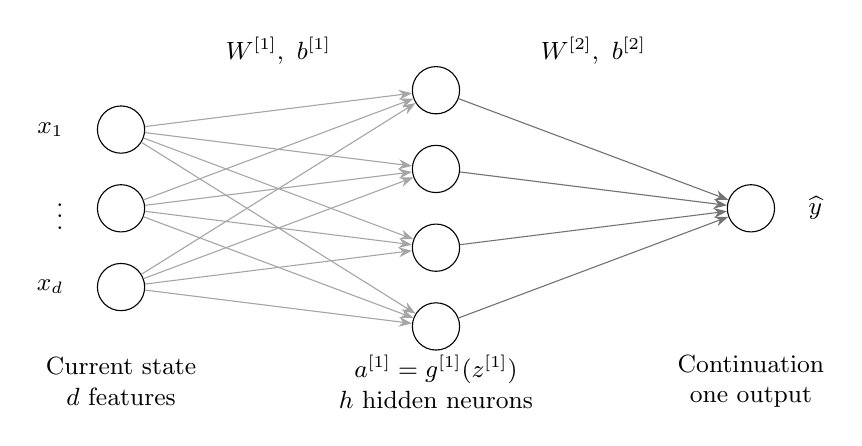
\begin{tikzpicture}[>=Stealth,unit/.style={circle,draw,minimum size=6mm,inner sep=0pt},
 every node/.style={font=\small}]
\foreach \i/\y in {1/1,2/0,3/-1}{\node[unit] (x\i) at (0,\y) {};}
\foreach \j/\y in {1/1.5,2/.5,3/-.5,4/-1.5}{\node[unit] (h\j) at (4,\y) {};}
\node[unit] (out) at (8,0) {};
\foreach \i in {1,2,3}{\foreach \j in {1,2,3,4}{\draw[->,black!35] (x\i)--(h\j);}}
\foreach \j in {1,2,3,4}{\draw[->,black!55] (h\j)--(out);}
\node[left=3mm of x1] {$x_1$};
\node[left=3mm of x2] {$\vdots$};
\node[left=3mm of x3] {$x_d$};
\node[right=3mm of out] {$\widehat y$};
\node at (2,2) {$W^{[1]},\ b^{[1]}$};
\node at (6,2) {$W^{[2]},\ b^{[2]}$};
\node[align=center] at (0,-2.2) {Current state\\$d$ features};
\node[align=center] at (4,-2.2) {$a^{[1]}=g^{[1]}(z^{[1]})$\\$h$ hidden neurons};
\node[align=center] at (8,-2.2) {Continuation\\one output};
\end{tikzpicture}
\caption{One observation through the continuation network. Only representative
neurons are drawn. All observations use the same weights at a given exercise date.
In the implementation, the input and output use the scaled units defined below.}
\end{figure}

\paragraph{Several observations.}
Stack the $M$ observations in $A^{[0]}\in\R^{M\times d}$. The same computation becomes
\[
 Z^{[1]}=A^{[0]}W^{[1]}+b^{[1]},\qquad
 A^{[1]}=g^{[1]}(Z^{[1]}),\qquad
 \widehat Y=A^{[1]}W^{[2]}+b^{[2]},
\]
with biases broadcast across rows. The dimensions are
\begin{center}
\begin{tabular}{lll}
\toprule
Quantity & Shape & Role\\
\midrule
$A^{[0]}$ & $M\times d$ & One row per observation\\
$W^{[1]},\ b^{[1]}$ & $d\times h,\ 1\times h$ & Hidden affine map\\
$Z^{[1]},\ A^{[1]}$ & $M\times h$ & Hidden pre-activations and activations\\
$W^{[2]},\ b^{[2]}$ & $h\times1,\ 1\times1$ & Output affine map\\
$\widehat Y$ & $M\times1$ & One continuation prediction per row\\
\bottomrule
\end{tabular}
\end{center}
The sample size changes the number of rows processed, not the weight dimensions.
For $d=50$ and $h=32$, $W^{[1]}$ has shape $(50,32)$ and $W^{[2]}$ has shape
$(32,1)$, whether training uses a thousand or a million paths. Here $M$ denotes
the total number of observations and $m$ indexes one observation. When fitting
only on in-the-money paths at date $t_n$, the input has $|I_n|$ rows.

\subsection{Parameter count and comparison criteria}
There are
\[
 dh+h+h+1=(d+2)h+1
\]
trainable parameters per fitted network. At $d=50$, a width of $32$ gives $1665$
parameters: more than a quadratic polynomial's $1326$, but fewer than a cubic
polynomial's $23426$. Hidden width is a separate choice from polynomial degree.
The jump from quadratic to cubic polynomial bases motivates testing a neural
alternative with a controlled width. At fixed width, its parameter count grows
linearly with $d$, and its hidden features are learned rather than prescribed.
This offers a different approximation budget, without guaranteeing a better
policy or a shorter training time.

The fitted networks enter the same policy evaluation as the polynomials.
Independent policy value, its uncertainty and stability across repetitions
remain the comparison criteria; regression MSE alone does not rank policies.

\subsection{Activation and scaling}
Following the numerical experiments of Lapeyre--Lelong~\cite{LL}, the hidden
activation is a leaky ReLU:
\[
 g^{[1]}(z)=\begin{cases}z,&z\geq0,\\0.3z,&z<0.\end{cases}
\]
Ordinary ReLU has zero derivative on the negative half-line. A hidden neuron
whose pre-activation is negative on every training observation contributes no
gradient to its incoming weights. Leaky ReLU preserves a nonzero activation
derivative there. This motivates its use, without establishing that it outperforms
ReLU in this problem or that the slope $0.3$ is optimal. The output remains linear;
its predictions are not constrained to be nonnegative. The positive-payoff
exercise condition in Section 3 still applies.

Both regression families use the fixed transformations
\begin{equation}\label{eq:scaling}
 \widetilde x=x/K-\mathbf 1,\qquad \widetilde Y_n=Y_n/K,
 \qquad \widehat c_n(x)=K f_{\widehat\theta_n}(x/K-\mathbf 1),
\end{equation}
with $\theta$ replaced by $\beta$ for the polynomial. Prices are centred at the
strike and targets are expressed in strike units. This reduces dependence of
optimization on the monetary units and brings near-the-money inputs closer to
zero. It is not variance standardization, and does not guarantee well-conditioned
features in every model. No statistics are re-estimated on validation or test data.
Predictions are converted back to monetary units before exercise decisions.
Scaling the target is distinct from discounting: $Y_n$ was already discounted to
time zero. For a full polynomial basis, the affine change of input preserves its
span; the exact least-squares problem is only reparametrized.

\subsection{Mini-batches, Adam and warm starts}
At a fixed exercise date, the future-policy cashflows $Y_n^{(m)}$ are held fixed
throughout training. The loss on a mini-batch $\mathcal B\subset I_n$ is
\[
 J_{\mathcal B}(\theta)=\frac1{|\mathcal B|}\sum_{m\in\mathcal B}
 \left(f_\theta(\widetilde X_n^{(m)})-\widetilde Y_n^{(m)}\right)^2.
\]
Backpropagation computes its gradient. An optimizer then updates the parameters
before the next batch. One epoch visits every eligible observation once, with
observations shuffled between epochs. Thus an epoch has
$\lceil |I_n|/B\rceil$ updates for batch size $B$, whereas full-batch descent has
one. Here $B$ denotes only the number of rows in a mini-batch; $M$ remains the
number of simulated paths. Mini-batches reduce memory for network activations
and computation per update, at the cost of a noisier gradient.

Adam~\cite{Adam} combines a moving average of gradients with a moving average
of their componentwise squares. If $g_k$ is the mini-batch gradient at update $k$,
its two accumulators, initially zero, satisfy
\[
 u_k=\beta_1u_{k-1}+(1-\beta_1)g_k,\qquad
 v_k=\beta_2v_{k-1}+(1-\beta_2)g_k^{\odot2}.
\]
After the initial-zero corrections $\widehat u_k=u_k/(1-\beta_1^k)$ and
$\widehat v_k=v_k/(1-\beta_2^k)$, the update is
\[
 \theta_{k+1}=\theta_k-\eta\,
 \frac{\widehat u_k}{\sqrt{\widehat v_k}+\varepsilon}.
\]
All operations in the fraction are componentwise. The first average smooths the
direction; the second adjusts the update scale for each parameter. The learning
rate $\eta$ is still a tuning choice. Adam neither changes the squared-error
objective nor guarantees its global minimum. The implementation uses
$\beta_1=0.9$, $\beta_2=0.999$ and $\varepsilon=10^{-8}$.

When moving backwards from date $n+1$ to $n$, the next network starts from the
previously fitted weights. Each date retains a separate fitted model, and Adam's
accumulators are reset. The fixed scaling in~\eqref{eq:scaling} keeps the meaning
of these weights consistent across dates. Nearby continuation functions may be
similar, making such a warm start useful, but shorter training must be assessed
numerically. Following Lapeyre--Lelong~\cite{LL}, a network trained from random
weights, at the last regression date, uses ten epochs, and a warm-started network
uses one epoch. The article reports that further passes did not reduce the training
error at earlier dates in its experiments; a variant with five epochs after each
warm start tests this in our setting. Widths are $32$ and $128$, with batch size
$256$ and learning rate $10^{-3}$. These are predeclared candidates, not optimized
hyperparameters, and not an exact replication of the article, which does not
specify every training detail.

\section{Implementation and experimental protocol}
\subsection{Code organization and numerical checks}
The notebook separates market simulation, payoffs, regression and exercise
decisions. A \texttt{BlackScholesModel} generates joint paths. Separate payoff
classes represent the one-asset put, geometric basket put and max-call.
The two regressors expose the same \texttt{fit} and \texttt{predict} interface,
allowing \texttt{LSMPricer} to use one backward recursion and one forward evaluation
for both methods. The neural model is an \texttt{nn.Module} with two
\texttt{nn.Linear} layers and a leaky ReLU between them. PyTorch stores the
linear weights transposed relative to the row-vector convention in
equation~\eqref{eq:network}; its forward operation implements the same affine map.

Polynomial fitting never stores the full design matrix. If $\Phi_k$ and $y_k$ contain
the rows of a block of paths, the normal equations are accumulated as
\[
 \Phi^\top\Phi=\sum_k\Phi_k^\top\Phi_k,\qquad \Phi^\top y=\sum_k\Phi_k^\top y_k,
\]
so memory depends on $q$ and on the block size, not on the number of paths.
At $d=50$ and degree two, $\Phi$ would occupy about $1.1$ GB for $10^5$ rows in
double precision, whereas $\Phi^\top\Phi$ occupies $14$ MB. The columns are rescaled
so that $\Phi^\top\Phi$ has a unit diagonal, and the system is solved through the
Cholesky factorization $\Phi^\top\Phi=LL^\top$. Forming $\Phi^\top\Phi$ squares the
condition number, $\kappa_2(\Phi^\top\Phi)=\kappa_2(\Phi)^2$, so rounding errors can be
amplified; a QR factorization of $\Phi$ avoids this, at a higher cost. The factorization
fails if the matrix is not numerically positive definite, and the condition number of
the rescaled matrix is recorded at each date. Rather than relying on a general threshold,
a check compares this solution with a direct least-squares solve based on a singular
value decomposition of $\Phi$ itself, on the bases with the largest condition numbers
observed in the study: the one-asset quartic, the five-asset bases of degrees four to six
and the fifty-asset quadratic. The check uses in-the-money states at the first and last
regression dates, with $10^4$ paths, the smallest training budget, where conditioning is
worst, and compares both the predictions and the resulting exercise decisions. The
predictions agree to within $3\times10^{-10}$, and no exercise decision changes.

Predictions are evaluated in blocks, and neural training processes mini-batches.
Paths use float32 storage; polynomial solves, discounted cashflows and Monte Carlo
sums use float64. Results are saved after every repetition, so that an interrupted
study resumes and tables and figures are rebuilt without recomputation.

The notebook contains executable checks with distinct purposes:
\begin{itemize}
 \item the eight-path example of Longstaff--Schwartz, using its published
 paths as reference data, checks the exercise recursion;
 \item recovery of a known polynomial, fitted over several blocks, checks the
 feature matrix, the solver and the monetary scaling, while network shapes and
 parameter counts check its interface;
 \item forward application on training paths is compared with the backward
 value, and each retained cashflow with the payoff at its stored exercise index;
 \item simulated log-return moments are inspected, and a European CRR put
 is compared with the Black--Scholes formula;
 \item on in-the-money states of the most ill-conditioned bases, at the first and last
 regression dates, the blockwise Cholesky solution is
 compared with a direct least-squares solve.
\end{itemize}
\subsection{Contracts and reference values}
The contracts are those of Lapeyre--Lelong~\cite[Tables 1, 3 and 9--11]{LL}:
a one-dimensional put, a geometric basket put with a scalar benchmark, and
dividend-paying max-calls. Parameters are shared across assets within each case,
with equicorrelation $\rho$.
\begin{center}
\small
\begin{tabular}{lrrrrrrrr}
\toprule
Contract & $d$ & $S_0^j$ & $K$ & $r$ & $\delta$ & $\sigma$ & $\rho$ & $(T,N)$\\
\midrule
Put & 1 & 100 & 110 & .10 & 0 & .25 & 0 & $(1,10)$\\
Geometric put & 10 & 100 & 100 & .05 & 0 & .20 & .20 & $(1,10)$\\
Max-call & 5 & 100 & 100 & .05 & .10 & .20 & 0 & $(3,9)$\\
Max-call & 50 & 100 & 100 & .05 & .10 & .20 & 0 & $(3,9)$\\
\bottomrule
\end{tabular}
\end{center}
The polynomial candidates have degrees two to four for the put, two and three for the
geometric basket, two to six for the five-asset max-call (six being the highest degree
reported by Lapeyre--Lelong for this contract), and one and two at fifty dimensions,
where the cubic basis would require $23426$ coefficients.

For the put, Lapeyre--Lelong use the benchmark $11.987$, a numerical value reported
as accurate to the digits shown. A Cox--Ross--Rubinstein (CRR) tree is also computed:
it refines the transition mesh but allows exercise only on the Bermudan dates, so
refining it approximates the same contract. Values with $500$, $1000$ and $2000$
substeps per exercise interval show the effect of refinement.

For the geometric basket $G_t=(\prod_{j=1}^dS_t^j)^{1/d}$, averaging log-prices
gives a scalar geometric Brownian motion with
\[
 \sigma_G^2=\frac1{d^2}\sigma^\top\Gamma\sigma,\qquad
 \delta_G=\frac1d\sum_j\delta_j
 +\frac1{2d}\sum_j\sigma_j^2-\frac12\sigma_G^2.
\]
Thus $dG_t=(r-\delta_G)G_t\,dt+\sigma_GG_t\,dB_t$. Under these constant coefficients,
the conditional law of future basket increments depends only on the present basket,
so observing the full asset vector adds no exercise information. The reduction is
exact; the same CRR tree then provides a numerical reference, while the regressors
still receive the ten asset prices.

No scalar reduction exists for the max-call. Lapeyre--Lelong quote the $95\%$
intervals $[26.14,26.17]$ for five assets and $[69.56,69.95]$ for fifty assets,
obtained by Becker et al.; they are not recomputed here. The prices tabulated by
Lapeyre--Lelong are estimated on the training paths, which can be optimistic;
they are points of comparison, not estimates directly comparable with independent
test values.

\subsection{Independent comparisons and uncertainty}
Each repetition uses independent training, validation and test samples, shared
between regression candidates: $M_{\rm train}=10^5$, $M_{\rm valid}=10^5$ and
$M_{\rm test}=10^6$ paths, the test paths being generated and evaluated in blocks
of $10^5$. There are $R=5$ repetitions.

Only training paths determine the fitted regressors and the time-zero decision.
At each date, validation paths provide cashflow targets under the already learned
future policy, permitting a held-out mean squared error. These targets are
independent of fitting that policy, but their variability includes irreducible
cashflow noise. Different policies may also produce different targets; their
MSEs are diagnostics rather than a direct ranking of policy values.

Within each family, the candidate with the highest validation policy value is
selected before any test path is simulated. The comparison of interest is between
the selected polynomial and the selected network; test values are also reported
for every candidate. For one frozen policy, an approximate conditional $95\%$
Monte Carlo interval is
\[
 \widehat V\ \pm\ 1.96\frac{s_H}{\sqrt{M_{\rm test}}},
 \qquad s_H^2=\frac1{M_{\rm test}-1}\sum_m(H^{(m)}-\widehat V)^2.
\]
For a comparison on common test paths, form
$D^{(m)}=H_{\rm neural}^{(m)}-H_{\rm polynomial}^{(m)}$ and use
$s_D/\sqrt{M_{\rm test}}$ for the standard error of their mean difference.
Ignoring this pairing would discard the covariance between the two payoffs.

These intervals treat the fitted policies as fixed. Retraining on new paths changes
the policies, and hence their values. If $\Delta_r$ denotes the mean paired
difference in repetition $r$, the comparison across repetitions is summarized by
\[
 \overline\Delta\ \pm\ t_{R-1,0.975}\,\frac{s_\Delta}{\sqrt R},
 \qquad s_\Delta^2=\frac1{R-1}\sum_{r=1}^R(\Delta_r-\overline\Delta)^2.
\]
This interval already contains the test noise of each $\Delta_r$, so the
within-repetition standard errors are reported separately rather than added to it.
With five repetitions it is approximate. No interval here bounds the shortfall from $V_0$.

Fitting times include the validation diagnostics but not the simulation of the training
and validation paths. The evaluation time, recorded separately and not reported here,
includes the simulation of the test blocks. These are indicative measurements on one
machine, not benchmarks.

\section{Numerical results}
\subsection{Checks and reference values}
All checks of Section~5.1 pass. The eight-path example returns $0.114434$, the
published value $0.1144$, with the published exercise dates. The European CRR price
differs from the Black--Scholes formula by $8\times10^{-4}$ with $200$ substeps per
interval, and the simulated log-return correlation is $0.396$ for a target of $0.4$.
The reference trees are stable under refinement:
\begin{center}
\begin{tabular}{lrrr}
\toprule
Substeps per exercise interval & $500$ & $1000$ & $2000$\\
\midrule
Put & $11.98798$ & $11.98735$ & $11.98748$\\
Geometric put & $2.92972$ & $2.92969$ & $2.92975$\\
\bottomrule
\end{tabular}
\end{center}
The put reference agrees with the value $11.987$ used by Lapeyre--Lelong.
Rerunning the five-asset case with additional candidates reproduced the values of
the common candidates to the digits reported.

\subsection{Policy values with $10^5$ training paths}
Figure~\ref{fig:values} shows the independent test value of every candidate, and
Table~\ref{tab:main} compares the policies selected by validation in each family.
\begin{figure}[ht]
\centering
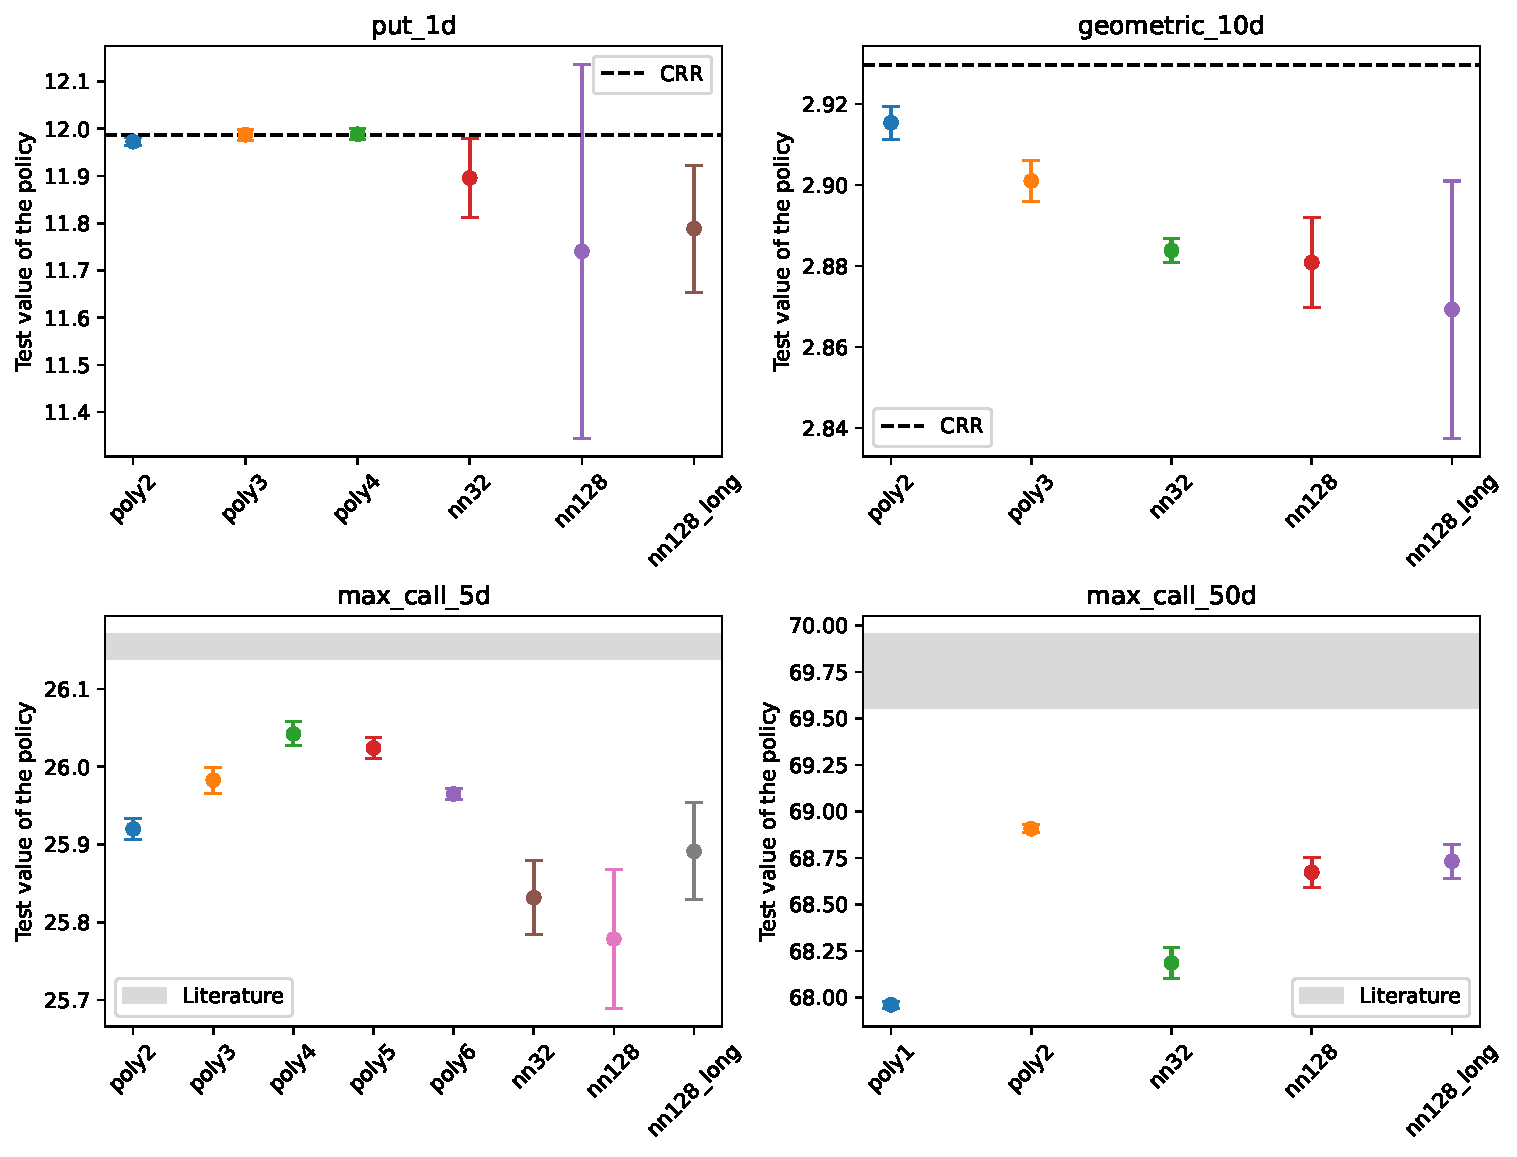
\includegraphics[width=\textwidth]{fig_policy_values_100000.pdf}
\caption{Test values of all candidates with $M_{\rm train}=10^5$: means over five
repetitions and $95\%$ Student half-widths. Dashed lines: CRR references; grey bands:
literature intervals.}\label{fig:values}
\end{figure}
\begin{table}[ht]
\centering
\small
\begin{tabular}{lcccc}
\toprule
Contract & Reference & Polynomial & Network & Network $-$ polynomial\\
\midrule
Put & $11.987$ & $11.988$ & $11.901$ & $-0.088\pm0.074$\\
Geometric put & $2.930$ & $2.915$ & $2.886$ & $-0.030\pm0.011$\\
Max-call, $d=5$ & $[26.14,26.17]$ & $26.032$ & $25.891$ & $-0.141\pm0.072$\\
Max-call, $d=50$ & $[69.56,69.95]$ & $68.907$ & $68.761$ & $-0.145\pm0.061$\\
\bottomrule
\end{tabular}
\caption{Selected policies with $M_{\rm train}=10^5$: mean test values over five
repetitions and paired differences with $95\%$ Student half-widths. The mean
within-repetition Monte Carlo standard errors of the differences are $0.004$,
$0.002$, $0.008$ and $0.008$.}\label{tab:main}
\end{table}

For the put, degrees three and four reach the reference within Monte Carlo error.
The networks are lower and less stable across repetitions; the width-128 network
varies widely, and validation retained the width-32 network in four repetitions out
of five. For the geometric basket, the full-state quadratic polynomial lies $0.014$
below the tree, and the cubic basis, with $286$ coefficients, is already worse.

For the five-asset max-call, the test value increases with the degree up to four and
then decreases,
\[
 25.920,\quad 25.983,\quad 26.042,\quad 26.024,\quad 25.965
 \qquad\text{for degrees }2,\ldots,6,
\]
while the training estimates keep increasing: $26.19$, $26.26$ and $26.36$ for degrees
four to six. The best degree is therefore inside the candidate set. At fifty assets,
the quadratic basis, the largest one available, remains ahead of every network.

In every contract the selected polynomial is ahead of the selected network, and the
interval across repetitions excludes zero, narrowly for the put. For the max-calls,
both families remain below the literature intervals, by about $0.1$ at five assets
and $0.65$ at fifty. The expected values of these policies are lower bounds for $V_0$,
and the Monte Carlo means estimate them; without an upper bound, the remaining gap to
$V_0$ cannot be split between the regressions and the reference.

\subsection{Training estimates and training effort}
Figure~\ref{fig:comparison} shows the paired differences of each repetition and the
mean gap between training estimates and test values of the selected policies.
\begin{figure}[ht]
\centering
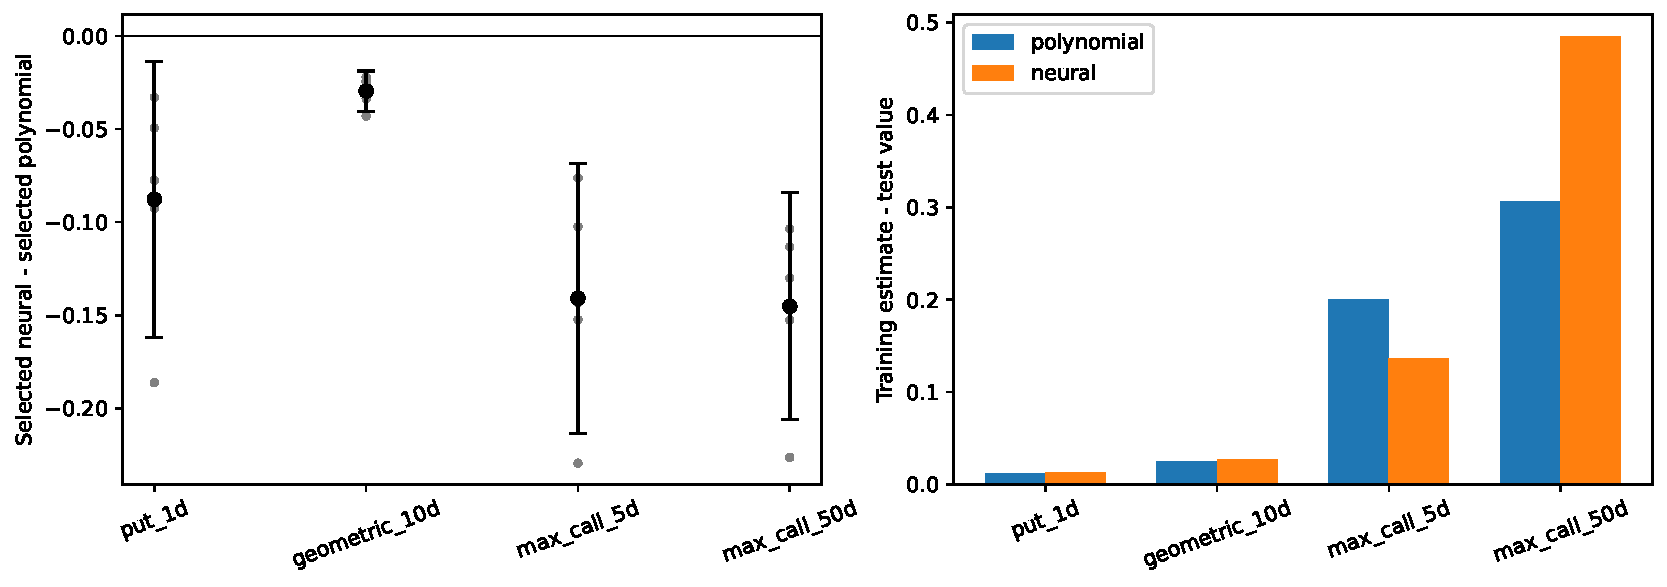
\includegraphics[width=\textwidth]{fig_comparison_100000.pdf}
\caption{Left: selected network minus selected polynomial, per repetition (grey) and
mean with $95\%$ Student interval. Right: training estimate minus test value of the
selected policies, $M_{\rm train}=10^5$.}\label{fig:comparison}
\end{figure}
The gaps are larger in high dimension: $0.012$ and $0.013$ for the put, $0.025$ and
$0.027$ for the geometric basket, $0.20$ and $0.14$ for the polynomial and the network at
five assets, $0.31$ and $0.48$ at fifty. Their intervals across repetitions appear in
Table~\ref{tab:budget}; those of the put are compatible with zero. At fifty assets the
ranking reverses between the two evaluations: the longer-trained network has a training
estimate of $69.30$ against $69.21$ for the quadratic polynomial, but test values of
$68.73$ against $68.91$. A comparison on training paths would have selected the wrong
family. In the first repetition at fifty assets, the polynomial also has the lower
held-out regression error at every date. This is a descriptive observation, not evidence
by itself: the two policies induce different targets, and a lower error may also reflect
less variable cashflows. Only the test values decide.

The variant trained for five epochs after each warm start, with about three times as
many updates, improves the five-asset max-call in all five repetitions, by $0.11$ on
average. At fifty assets the average change is $+0.06$ with $10^5$ paths and $+0.004$ with
$10^6$, but the differences take both signs across repetitions and reach $0.32$ in absolute
value with $10^6$ paths. Additional epochs thus help in the five-asset case; elsewhere their
effect is not resolved, and the network value varies substantially from one training to
another. Larger samples also bring more updates per epoch, so the two effects cannot be
separated here; the number of updates is only one aspect of training, together with the
learning rate, the batch size and the initialization.

\subsection{Effect of the training budget}
The whole study was repeated with $10^4$ training paths, and the fifty-asset case with
$10^6$, keeping $10^5$ validation and $10^6$ test paths.
\begin{table}[ht]
\centering
\footnotesize
\setlength{\tabcolsep}{4pt}
\begin{tabular}{lrccccc}
\toprule
Contract & $M_{\rm train}$ & Polynomial & Network & Net. $-$ poly. & Gap poly. & Gap net.\\
\midrule
Put & $10^4$ & $11.985$ & $11.904$ & $-0.081\pm0.033$ & $-0.014\pm0.076$ & $-0.040\pm0.087$\\
 & $10^5$ & $11.988$ & $11.901$ & $-0.088\pm0.074$ & $+0.012\pm0.015$ & $+0.013\pm0.018$\\
Geometric put & $10^4$ & $2.872$ & $2.850$ & $-0.022\pm0.038$ & $+0.145\pm0.027$ & $+0.044\pm0.039$\\
 & $10^5$ & $2.915$ & $2.886$ & $-0.030\pm0.011$ & $+0.025\pm0.014$ & $+0.027\pm0.019$\\
Max-call, $d=5$ & $10^4$ & $25.887$ & $25.858$ & $-0.030\pm0.049$ & $+0.125\pm0.356$ & $+0.046\pm0.399$\\
 & $10^5$ & $26.032$ & $25.891$ & $-0.141\pm0.072$ & $+0.200\pm0.139$ & $+0.136\pm0.112$\\
Max-call, $d=50$ & $10^4$ & $67.927$ & $68.683$ & $+0.756\pm0.126$ & $+0.205\pm0.151$ & $+0.820\pm0.490$\\
 & $10^5$ & $68.907$ & $68.761$ & $-0.145\pm0.061$ & $+0.306\pm0.064$ & $+0.484\pm0.165$\\
 & $10^6$ & $68.993$ & $68.823$ & $-0.170\pm0.159$ & $+0.018\pm0.018$ & $+0.120\pm0.035$\\
\bottomrule
\end{tabular}
\caption{Selected policies for several training budgets: mean test values, paired
differences with $95\%$ Student half-widths, and mean gaps between training estimates
and test values. All intervals are $95\%$ Student half-widths across the five
repetitions.}\label{tab:budget}
\end{table}
\begin{figure}[ht]
\centering
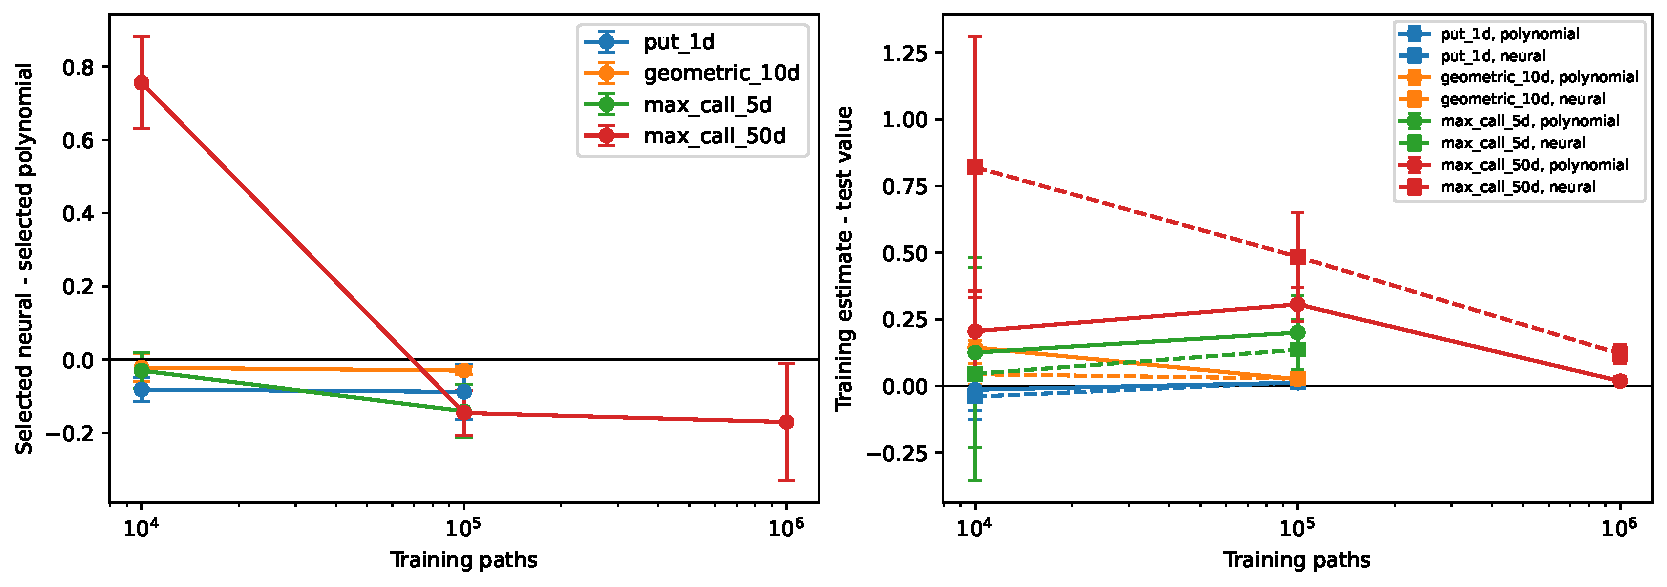
\includegraphics[width=\textwidth]{fig_budget.pdf}
\caption{Effect of the number of training paths on the selected difference (left) and
on the gap between training estimates and test values (right).}\label{fig:budget}
\end{figure}

With $10^4$ paths at fifty assets, the quadratic basis has about seven observations
per coefficient. Its training estimate reaches $71.09$, above the literature interval,
while its test value is $67.73$. Validation therefore retains the linear basis, and the
network leads by $0.76$. From $10^5$ paths the quadratic basis can be estimated and the
polynomial leads again; with $10^6$ paths it gains $0.09$, the network $0.06$, and the
difference remains negative, although its interval nearly reaches zero. The same effect
appears at five assets with $10^4$ paths: from degree two to six, the training estimates
rise from $26.01$ to $27.66$ while the test values fall from $25.89$ to $25.13$, and
validation retains degree two.

The gaps of Table~\ref{tab:budget} are themselves estimates, summarized like the other
quantities by their dispersion across repetitions. The policy is fitted on the training
paths, so a standard error computed on those same paths would not be justified. The
intervals across repetitions avoid this; with five repetitions they remain approximate.
The gaps of the put at both budgets, and of the five-asset max-call with $10^4$ paths, are
compatible with zero: these experiments do not exhibit a bias, which is not the same as
showing that there is none. The gaps of the geometric basket and of the fifty-asset
max-call are clearly positive.

Conditionally on the training data, the test average is unbiased for the value of the
selected policy, so the expected gap equals the optimism of the training estimate; the
suboptimality of the policy affects both evaluations and cancels. In fifty dimensions,
the gap of the selected polynomial follows the ratio $q/M$ between the number of
coefficients and the number of paths: $+0.018$ at $q/M=0.0013$, $+0.205$ at $0.0051$ and
$+0.306$ at $0.0133$. This is an observation, not an isolated effect: the selected degree
and the budget change together.

\paragraph{Computational cost.}
Median fitting times, including the validation diagnostics, illustrate the scaling.
For the put, a polynomial takes $0.4$ seconds and a network $10$ to $35$ seconds. At fifty
assets with $10^5$ paths, the quadratic polynomial takes $96$ seconds and the networks
$20$ to $59$ seconds; with $10^6$ paths, $300$ seconds against $56$ to $155$ seconds.
The polynomial is much cheaper in low dimension, while its cost grows faster with the
dimension. These are measurements on one laptop CPU, not benchmarks.

\section{Conclusion}
The Longstaff--Schwartz recursion was implemented with two interchangeable regressors
and evaluated on independent paths. Its polynomial version reproduces the published
eight-path example and the one-dimensional reference value. Because every learned policy
has a value below $V_0$, the two regressors were compared through their test values,
with paired differences on common paths and five independent repetitions.

With $10^5$ training paths and more, the policy selected among polynomial bases is ahead
of the policy selected among one-hidden-layer networks in all four contracts, by $0.03$
to $0.17$, including at fifty assets where the quadratic basis is the largest feasible
one. The ranking depends on the amount of data: with $10^4$ paths at fifty assets, the
quadratic basis cannot be estimated reliably and the network leads. Estimates computed
on training paths are optimistic in high dimension and with little data, and can reverse
the ranking of the two families; independent evaluation is therefore essential.
Additional epochs after each warm start improved the five-asset network; at fifty assets
their effect was not resolved.

These conclusions concern the tested recipes. Deeper networks, used in part by
Lapeyre--Lelong, and other training schedules were not explored, and the network values
vary markedly from one training to another. Five repetitions give approximate intervals,
and the timings are indicative. For the max-calls, no upper bound
was computed, so the gap to the literature intervals, about $0.1$ at five assets and
$0.65$ at fifty, remains unexplained. Dual upper bounds and deeper or better trained
networks are the natural extensions.


\clearpage
\phantomsection
\addcontentsline{toc}{section}{References}
\begin{thebibliography}{9}
\bibitem{LS} F. A. Longstaff and E. S. Schwartz (2001).
Valuing American options by simulation: a simple least-squares approach.
\emph{The Review of Financial Studies}, 14(1), 113--147.
\bibitem{LL} B. Lapeyre and J. Lelong (2020).
Neural network regression for Bermudan option pricing.
\emph{arXiv:1907.06474v3}. \url{https://arxiv.org/abs/1907.06474v3}.
\bibitem{Adam} D. P. Kingma and J. Ba (2015).
Adam: A method for stochastic optimization.
\emph{International Conference on Learning Representations}.
\url{https://arxiv.org/abs/1412.6980}.
\end{thebibliography}
\end{document}
